\documentclass[data,datadescriptor,submit,moreauthors,pdftex]{Definitions/mdpi}
\microtypesetup{expansion=false}

\usepackage{amsmath,amssymb}
\usepackage{booktabs,tabularx,array,ragged2e,longtable}
\usepackage{graphicx}
\usepackage{tikz}
\usetikzlibrary{arrows.meta,positioning,fit,calc}
\usepackage{enumitem}
\usepackage{float}
\usepackage{xurl}
\usepackage{listings}
\setlength{\headheight}{25pt}
\setlength{\emergencystretch}{2em}
\newcolumntype{L}{>{\RaggedRight\arraybackslash}X}
\newcolumntype{P}[1]{>{\RaggedRight\arraybackslash}p{#1}}
\newcommand{\datasetname}{Chile-ED-Resp}
\newcommand{\datasetversion}{1.0.0}
\newcommand{\dataseturl}{https://github.com/cvidalmsu/chile-ed-resp-benchmark}
\newcommand{\datasetdoi}{10.5281/zenodo.REPLACE-AFTER-RELEASE}
\newcommand{\sourceid}{ae6c9887-106d-4e98-8875-40bf2b836041}
\renewcommand{\today}{August 7, 2026}
\lstset{basicstyle=\ttfamily\footnotesize,breaklines=true,frame=single,columns=fullflexible,showstringspaces=false}

\firstpage{1}
\makeatletter
\setcounter{page}{\@firstpage}
\makeatother
\pubvolume{1}
\issuenum{1}
\articlenumber{0}
\pubyear{2026}
\copyrightyear{2026}
\datereceived{}
\dateaccepted{}
\datepublished{}
\hreflink{https://doi.org/}

\Title{Chile-ED-Resp: A Curated and Reproducible Weekly Hospital Dataset for Respiratory Emergency-Demand Forecasting in Chile}
\TitleCitation{Chile-ED-Resp: A Curated Weekly Hospital Dataset for Respiratory Emergency-Demand Forecasting}

\Author{Wilman Balc\'azar-Quimi~$^{1}$, Carla Angulo~$^{2,*}$, Cristian Cornejo-Gaete~$^{3}$, Brandon Salinas-Neira~$^{2}$, Jorge Fern\'andez-Bast\'ias~$^{2}$, Miguel Tupac-Yupanqui~$^{4}$, and Cristian Vidal-Silva~$^{5,*}$}
\AuthorNames{Wilman Balc\'azar-Quimi, Carla Angulo, Cristian Cornejo-Gaete, Brandon Salinas-Neira, Jorge Fern\'andez-Bast\'ias, Miguel Tupac-Yupanqui and Cristian Vidal-Silva}
\AuthorCitation{Balc\'azar-Quimi, W.; Angulo, C.; Cornejo-Gaete, C.; Salinas-Neira, B.; Fern\'andez-Bast\'ias, J.; Tupac-Yupanqui, M.; Vidal-Silva, C.}
\address{%
$^{1}$ \quad Facultad de Salud y Servicios Sociales, Universidad Estatal de Milagro, Milagro 092301, Guayas, Ecuador; wbalcazarq@unemi.edu.ec\\
$^{2}$ \quad Escuela de Ciencias Digitales y Tecnolog\'ias Avanzadas, Universidad Bernardo O'Higgins, Santiago 8370846, Chile; carla.angulo@ubo.cl, \{brandon.salinas, jorge.fernandez\}@pregrado.ubo.cl\\
$^{3}$ \quad Facultad de Ingenier\'ia, Ciencia y Tecnolog\'ia, Universidad Bernardo O'Higgins, Santiago 8370846, Chile; cristian.cornejo@ubo.cl\\
$^{4}$ \quad EAP Ingenier\'ia de Sistemas e Inform\'atica, Universidad Continental, Huancayo 12000, Peru; mtupac@continental.edu.pe\\
$^{5}$ \quad Facultad de Ingenier\'ia y Negocios, Universidad de Las Am\'ericas, Manuel Montt 948, Providencia, Santiago~7500975, Chile; cristian.vidal.silva@edu.udla.cl}
\corres{Correspondence: carla.angulo@ubo.cl (C.A.); cristian.vidal.silva@edu.udla.cl (C.V.-S.)}

\abstract{Respiratory emergencies create recurrent seasonal pressure on hospital services, yet reproducible forecasting research is often hindered by the effort required to retrieve, interpret, harmonize, and document public administrative data. Chile-ED-Resp is a curated secondary dataset and reproducible processing pipeline derived from the official Chilean Ministry of Health/DEIS dataset ``Atenciones de urgencias de causas respiratorias por semana epidemiol\'ogica'', produced by the Sistema de Atenci\'on Diaria de Urgencias (SADU). The release focuses on the closed 2022--2025 period and retains official hospital emergency-unit records, respiratory cause labels, total counts, five age strata, establishment characteristics, geographic descriptors, and health-service identifiers. Two complementary analysis-ready artifacts are produced: a long table that preserves official count observations and a hospital-week forecasting table centered on high respiratory infection (IRA Alta), with selected respiratory causes pivoted as covariates. Only deterministic derivatives are added, including coverage diagnostics, chronological train/test labels, seasonal encodings, lags, and prior rolling means; official count fields are neither imputed nor smoothed. Reproducibility is supported through source retrieval metadata, SHA-256 checksums, a machine-readable data dictionary, cause and hospital-coverage inventories, automated validation, unit tests, and a GitHub Actions workflow that rebuilds the release from the official Parquet resource. The resource is intended to provide a transparent foundation for forecasting, benchmarking, health-informatics teaching, and secondary analyses while preserving provenance and the licensing conditions of the government source.}

\dataset{\datasetname{}, version \datasetversion{}. Creator: Balc\'azar-Quimi, W.; Angulo, C.; Cornejo-Gaete, C.; Salinas-Neira, B.; Fern\'andez-Bast\'ias, J.; Tupac-Yupanqui, M.; Vidal-Silva, C. Publisher/location: GitHub, \url{\dataseturl}. A versioned Zenodo DOI will be added to the archived release before journal publication: \texttt{\datasetdoi}.}
\datasetlicense{Curated data files: Creative Commons Attribution-NonCommercial 2.0 Generic (CC BY-NC 2.0), preserving the licensing conditions linked by the official source portal; software: MIT License.}
\keyword{emergency department; respiratory illness; hospital demand; time series; forecasting; data curation; DEIS; SADU; reproducibility; FAIR data; Chile}

\begin{document}

\section{Summary}
\label{sec:summary}

Hospital emergency departments must absorb demand that changes with epidemiological conditions, season, age structure, and local service organization. Respiratory illness is particularly relevant because recurrent winter epidemics can concentrate consultations and hospitalizations within a limited number of weeks. Forecasting approaches have consequently been used to anticipate emergency attendance, bed demand, and severe respiratory hospitalizations \citep{Lucini2020,Duarte2021,Albrecht2024,Ackermann2025}. Recent systematic evidence also shows growing use of machine-learning and deep-learning methods for emergency-demand prediction, while emphasizing persistent limitations in validation, data documentation, and transportability \citep{Blanco2025}. In Chile, regional analyses have reported marked temporal variation in emergency consultations and substantial respiratory-season effects \citep{ToroCastillo2024,DiazCarvajal2025}.

Within this setting, the Chilean Ministry of Health makes weekly respiratory emergency data publicly available through the Departamento de Estad\'isticas e Informaci\'on de Salud (DEIS). The source dataset, produced from the Sistema de Atenci\'on Diaria de Urgencias (SADU), reports consultations and hospitalizations by respiratory cause, establishment, statistical week, and age group \citep{DEIS2026,DEISDictionary2024}. Although the source is highly valuable, downstream forecasting studies must repeatedly solve the same data-engineering tasks: retrieving a large Parquet file, harmonizing field names and types, isolating hospital emergency units, separating consultations from hospitalization rows, checking temporal coverage, pivoting causes to hospital-week features, constructing lagged predictors without leakage, and documenting provenance.

From a data-publication perspective, the principal contribution of \datasetname{} is therefore not a new predictive algorithm. Instead, the resource provides a transparent and reusable data infrastructure derived from the official source. A closely related data-publication strategy has recently been demonstrated in \textit{Data} by Voinea and Voinea, who transformed heterogeneous national health-administration workbooks into harmonized artifacts with provenance logs, checksums, dictionaries, and a reproducible Python pipeline \citep{Voinea2026}. Other recent Data Descriptors likewise emphasize that dataset value depends on clear variable documentation, access conditions, and intended reuse rather than on inferential novelty alone \citep{Berth2026}. The design also follows the FAIR principles of findability, accessibility, interoperability, and reusability \citep{Wilkinson2016}.

Accordingly, \datasetname{} releases two complementary representations of the same official 2022--2025 respiratory emergency information. The first is a curated long-format table that preserves all qualifying hospital emergency-unit records and the official count values. The second is a forecasting-ready hospital-week table that reorganizes selected consultation causes into columns and adds only deterministic time-series features. An explicit coverage criterion identifies establishments suitable for benchmarking rather than hard-coding a small set of hospitals. The repository records the exact dimensions, hospital inventory, cause inventory, source checksum, retrieval timestamp, and validation results for each release, allowing later versions to remain auditable even if the upstream public portal revises historical records.

\section{Data Description}
\label{sec:data-description}

\subsection{Official Source and Scope}

The upstream resource is the government dataset \textit{Atenciones de urgencias de causas respiratorias por semana epidemiol\'ogica}, published through datos.gob.cl by the Chilean Ministry of Health/DEIS \citep{DEIS2026}. The active Parquet resource has identifier \texttt{\sourceid}. At the time this descriptor was prepared, the portal reported weekly updates and linked the resource to the Creative Commons Attribution-NonCommercial 2.0 Generic license \citep{CreativeCommonsBYNC20}. Because the current epidemiological year is continuously updated, the curated release intentionally uses the closed four-year interval 2022--2025. Restricting the versioned release to completed calendar years avoids treating a partially reported current week as a genuine demand decline.

The source schema contains 25 variables after normalization to snake-case names. These fields describe establishment, region, municipality, health service, establishment type, administrative dependency, level of care, emergency-care type, coordinates, complexity level, year, statistical week, cause code/order, cause label, total count, and five age-specific count fields. The public schema and representative field types have independently been demonstrated using the same DEIS resource in an open data-analysis workshop, supporting the reproducibility of the field mapping used here \citep{DEISDictionary2024}.

\begin{table}[H]
\caption{Variable families retained from the official DEIS/SADU source. The complete machine-readable dictionary is distributed as \texttt{metadata/data\_dictionary.csv}.}
\label{tab:source-fields}
\centering
\begin{tabularx}{\linewidth}{P{0.24\linewidth}P{0.36\linewidth}L}
\toprule
Family & Main fields & Interpretation \\
\midrule
Establishment & \texttt{establecimiento\_codigo}, \texttt{establecimiento\_glosa}, \texttt{tipo\_establecimiento}, \texttt{nivel\_atencion}, \texttt{nivel\_complejidad} & Official identifiers and service characteristics. \\
Geography & \texttt{region\_*}, \texttt{comuna\_*}, \texttt{latitud}, \texttt{longitud} & Administrative and geographic descriptors. \\
Health service & \texttt{servicio\_salud\_*}, \texttt{dependencia\_administrativa}, \texttt{tipo\_urgencia} & Network and emergency-unit descriptors. \\
Time & \texttt{anio}, \texttt{semana\_estadistica} & Official year and statistical/epidemiological week. \\
Respiratory event & \texttt{orden\_causa}, \texttt{causa}, \texttt{num\_total} & Cause label and total consultations or hospitalizations in the stratum. \\
Age strata & \texttt{num\_menor1anio}, \texttt{num1a4anios}, \texttt{num5a14anios}, \texttt{num15a64anios}, \texttt{num65o\_mas} & Official age-specific counts. \\
\bottomrule
\end{tabularx}
\end{table}

\subsection{Released Artifacts}

The repository generates the artifacts summarized in Table~\ref{tab:artifacts}. Exact row counts, numbers of establishments, numbers of causes, and file hashes are written at build time to \texttt{metadata/release\_metadata.json}, \texttt{metadata/hospital\_coverage.csv}, \texttt{metadata/causes.csv}, and \texttt{metadata/SHA256SUMS.txt}. Storing these quantities with the release is deliberate: the source is maintained by an external public agency and may undergo retrospective corrections, whereas a versioned research dataset must remain traceable to the precise snapshot used to build it.

\begin{table}[H]
\caption{Principal files created by the reproducible release pipeline.}
\label{tab:artifacts}
\centering
\begin{tabularx}{\linewidth}{P{0.37\linewidth}P{0.18\linewidth}L}
\toprule
File & Format & Role \\
\midrule
\texttt{chile\_ed\_resp\_hospital\_long} & Parquet; CSV.gz & Curated long-format hospital emergency-unit observations with official count fields plus provenance and quality-control variables. \\
\path{chile_ed_resp_ira_alta_forecasting} & Parquet; CSV & One row per hospital-week for selected respiratory consultation causes and deterministic forecasting features. \\
\texttt{source\_manifest.json} & JSON & Retrieval timestamp, upstream identifiers, source URL, byte size, SHA-256 checksum, and license metadata. \\
\texttt{release\_metadata.json} & JSON & Version, period, row/column counts, hospital/cause counts, curation rules, and transformation statements. \\
\texttt{hospital\_coverage.csv} & CSV & IRA Alta temporal coverage by establishment and benchmark recommendation flag. \\
\texttt{causes.csv} & CSV & Inventory of official cause labels, measure type, row count, and reported totals. \\
\texttt{validation\_checks.csv} & CSV & Machine-readable results of structural and quality-control checks. \\
\bottomrule
\end{tabularx}
\end{table}

\subsection{Curated Long Table}

The long table restricts the official source to the years 2022--2025, establishments classified as \texttt{Hospital}, and records whose emergency type contains the hospital-emergency designation \texttt{UEH}. No respiratory cause is removed at this stage. Consultation and hospitalization rows are distinguished from the official cause label and stored in the derived field \texttt{measure\_type}; this separation prevents hospitalization counts from being inadvertently interpreted as consultation-demand predictors.

Beyond normalization of column names and coordinate types, official count fields are retained unchanged. Derived fields include a deterministic row identifier, a human-readable year-week label, the fixed source-resource identifier, the sum of the five official age strata, the difference between that age sum and \texttt{num\_total}, and a quality flag. Any discrepancy between official totals and age-specific fields is reported rather than silently corrected. Likewise, missing source values remain missing; the release does not fill gaps through mean/median substitution, interpolation, or model-based imputation.

\subsection{Forecasting-Ready Hospital-Week Table}

For reuse in time-series forecasting, consultation rows are mapped to canonical variables using transparent text rules on official cause labels. The current mapping recognizes high respiratory infection (IRA Alta), influenza, pneumonia, acute bronchitis/bronchiolitis, other respiratory causes, identified COVID-19, and unidentified COVID-19 when those labels are present in the source. The mapping does not alter values: where multiple official rows map to the same hospital-week feature, their reported \texttt{num\_total} values are summed; where a feature is absent, the resulting cell remains missing rather than being replaced with zero.

Hospital selection for benchmarking is coverage-based. For each establishment, the pipeline counts weeks in which IRA Alta is observed and divides this value by the number of distinct IRA Alta year-week pairs available nationally within the release window. Establishments with coverage of at least 95\% receive \texttt{recommended\_for\_benchmark = True}. Researchers can therefore reproduce the recommended cohort or choose a different threshold without changing the curated long table.

Temporal features are constructed after sorting observations by hospital, year, and week. The release provides one-, two-, and four-week lags of IRA Alta, together with a previous-year same-week seasonal lag, trailing four- and 12-week means computed strictly from prior observations, and sine/cosine encodings of statistical week. A default chronological split labels 2022--2024 as training and 2025 as testing. Because lagged and rolling fields use only preceding values, the prepared table avoids look-ahead leakage by construction \citep{Hyndman2021}.

\section{Methods}
\label{sec:methods}

\subsection{Reproducible Processing Workflow}

Figure~\ref{fig:pipeline} summarizes the curation workflow. The process begins from the stable government resource identifier rather than from a manually downloaded local copy. The downloader uses repeated HTTP attempts and a command-line fallback, verifies that the retrieved object has a valid Parquet signature, computes a SHA-256 digest, and writes a source manifest before transformation. The raw government file is intentionally excluded from Git version control; the release instead stores its provenance metadata and redistributes only the curated 2022--2025 artifacts under the source-compatible license.

\begin{figure}[H]
\centering
\resizebox{0.98\linewidth}{!}{%
\begin{tikzpicture}[
node distance=0.55cm and 0.55cm,
box/.style={draw, rounded corners=3pt, align=center, minimum height=1.0cm, text width=2.7cm, fill=gray!7, font=\small},
arrow/.style={-Latex, thick}
]
\node[box] (source) {Official DEIS/SADU\\Parquet resource};
\node[box, right=of source] (prov) {Retrieval + SHA-256\\source manifest};
\node[box, right=of prov] (filter) {2022--2025\\Hospital + UEH};
\node[box, right=of filter] (long) {Curated long table\\official counts preserved};
\node[box, below=0.65cm of filter] (pivot) {Cause mapping +\\hospital-week pivot};
\node[box, left=of pivot] (features) {Coverage + lags +\\rolling/time features};
\node[box, left=of features] (valid) {Validation + inventories\\+ file checksums};
\node[box, left=of valid] (release) {GitHub/Zenodo\\versioned release};
\draw[arrow] (source) -- (prov);
\draw[arrow] (prov) -- (filter);
\draw[arrow] (filter) -- (long);
\draw[arrow] (long.south) |- (pivot.east);
\draw[arrow] (pivot) -- (features);
\draw[arrow] (features) -- (valid);
\draw[arrow] (valid) -- (release);
\end{tikzpicture}%
}
\caption{Reproducible Chile-ED-Resp curation workflow. All demand counts originate in the official DEIS/SADU resource; the pipeline adds deterministic organizational, provenance, quality-control, and forecasting fields.}
\label{fig:pipeline}
\end{figure}

\subsection{Schema Harmonization and Type Treatment}

Column names are normalized to lower-case snake case. Because public-data schemas can appear with either CamelCase or previously cleaned headings, the build script matches fields through an underscore-insensitive canonical key before checking for the complete expected 25-field schema. If an expected source field is absent, the build stops rather than guessing a replacement. Numeric count, year, week, and cause-order columns are explicitly parsed; coordinates are converted from decimal-comma text to numeric decimal-point representation. No other source values are standardized in a way that changes their substantive meaning.

The curation script also keeps an explicit cause inventory. The inventory records every official cause label present in the selected hospital/UEH period, its consultation/hospitalization classification, number of source rows, and aggregate reported total. Maintaining the original label alongside canonical forecasting features allows users to audit the text mapping and to rebuild alternative targets.

\subsection{Hospital Coverage and Selection}

Rather than selecting hospitals on the basis of peak demand, geographic convenience, or prior model performance, the release applies a transparent completeness criterion. Let $W$ denote the set of distinct year-week combinations in which IRA Alta is observed anywhere in the hospital subset, and let $W_h$ denote the subset observed for hospital $h$. Coverage is
\begin{equation}
C_h = \frac{|W_h|}{|W|}.
\end{equation}
The default benchmark recommendation is $C_h \geq 0.95$. The threshold is not presented as a clinical quality criterion; it is a data-completeness rule intended to reduce avoidable missingness in forecasting comparisons. The full hospital subset remains available so that users may adopt other inclusion criteria.

\subsection{Feature Engineering Without Leakage}

For a hospital $h$ and ordered weekly target series $y_{h,t}$, lag features are defined as $y_{h,t-k}$ for $k \in \{1,2,4,52\}$. Prior rolling means use
\begin{equation}
\bar{y}^{(m)}_{h,t}=\frac{1}{m}\sum_{j=1}^{m}y_{h,t-j}, \quad m \in \{4,12\},
\end{equation}
whenever all required prior values exist. The current observation $y_{h,t}$ is excluded from each rolling feature. Seasonal position is encoded as
\begin{equation}
s_t=\sin\left(\frac{2\pi w_t}{52}\right), \qquad c_t=\cos\left(\frac{2\pi w_t}{52}\right),
\end{equation}
where $w_t$ is statistical week. Such deterministic temporal encodings permit use by linear, tree-based, or neural forecasting models without adding external information.

\subsection{Automated Build and Versioning}

The public repository contains Python scripts for source retrieval, curation, validation, and an optional seasonal-naive baseline. Unit tests cover schema normalization and cause-label mapping. A manual GitHub Actions workflow installs the declared dependencies, executes the tests, downloads the official resource, builds both data artifacts, runs validation, and commits the versioned outputs and metadata. This approach makes the publication package independently rebuildable without requiring authors to distribute the large upstream raw file.

Version-specific provenance is strengthened through cryptographic hashes. The source manifest records retrieval time, file size, and SHA-256 of the official Parquet snapshot; the final checksum file records hashes of the curated Parquet/CSV artifacts and principal metadata files. Similar checksum-based provenance has recently been used in a national health-data Data Descriptor to distinguish an immutable research release from mutable upstream public files \citep{Voinea2026}.

\subsection{Technical Validation}

Validation is designed to detect structural and source-quality issues without rewriting official observations. Table~\ref{tab:validation} lists the automated checks. A \texttt{FAIL} status stops the release when the forecasting table cannot be trusted structurally; a \texttt{WARN} status exposes a potentially relevant anomaly while preserving the source values for transparent secondary analysis.

\begin{table}[H]
\caption{Automated validation checks implemented in \texttt{scripts/validate\_dataset.py}.}
\label{tab:validation}
\centering
\begin{tabularx}{\linewidth}{P{0.32\linewidth}P{0.16\linewidth}L}
\toprule
Check & Severity & Purpose \\
\midrule
Official source counts preserved & Pass assertion & Confirms that demand counts are read from DEIS/SADU and only derived fields are computed. \\
Analysis years & Fail if invalid & Ensures the versioned release is restricted to 2022--2025. \\
Non-negative counts & Warning & Reports unexpected negative administrative counts without silently changing them. \\
Age-total reconciliation & Warning & Compares \texttt{num\_total} with the five age-stratum fields and reports mismatches. \\
Unavailable age reconciliation & Warning & Reports rows for which the age check cannot be completed because source strata are missing. \\
Duplicate source strata & Warning & Flags repeated hospital-week-cause keys before wide aggregation. \\
Unique hospital-week forecast key & Fail if violated & Guarantees one forecasting row per establishment/year/week. \\
Chronological ordering & Warning & Verifies stable time ordering within the release. \\
Chronological split & Fail if violated & Ensures training years precede the 2025 test year. \\
No count imputation & Pass assertion & Documents that missing official counts are not replaced. \\
\bottomrule
\end{tabularx}
\end{table}

In addition to these checks, the pipeline writes the hospital-coverage table and cause inventory so that the cohort and mappings can be inspected independently of the manuscript. An optional seasonal-naive example predicts 2025 IRA Alta from the 52-week lag for recommended hospitals and writes establishment-level MAE, RMSE, and MAPE. Those metrics are intentionally treated as a usage demonstration rather than as a substantive result of the Data Descriptor.

\section{User Notes}
\label{sec:user-notes}

\subsection{Reproducing the Release}

Users can reproduce the complete release from a clean checkout with the commands below. Python 3.12 is used in the GitHub Actions workflow, while package versions are constrained through minimum versions in \texttt{requirements.txt}.

\begin{lstlisting}[language=bash]
git clone https://github.com/cvidalmsu/chile-ed-resp-benchmark.git
cd chile-ed-resp-benchmark
python -m venv .venv
# activate the environment for the operating system in use
pip install -r requirements.txt
pytest -q
python scripts/make_release.py --start-year 2022 --end-year 2025 --force-download
\end{lstlisting}

Alternatively, repository maintainers can run \textit{Actions $\rightarrow$ Build DEIS-SADU dataset $\rightarrow$ Run workflow}. The action records the newly retrieved source checksum before rebuilding the release. For a publication snapshot, users should cite the Zenodo DOI associated with the tagged GitHub release rather than a mutable branch URL.

\subsection{Recommended Forecasting Use}

For comparable model experiments, the recommended starting point is the forecasting artifact:
\begin{center}
\path{data/chile_ed_resp_ira_alta_forecasting.parquet}
\end{center}
Users should initially restrict the table to establishments carrying the benchmark recommendation flag. The supplied \texttt{split} field provides a simple 2022--2024/2025 holdout. Researchers requiring robust model comparison should additionally use rolling-origin or expanding-window validation inside the training period rather than randomly shuffling weekly observations \citep{Hyndman2021}. High-dimensional models should be interpreted cautiously because model complexity and sample frequency can materially affect performance in emergency-demand forecasting \citep{Tuominen2022,Blanco2025}.

For epidemiological or descriptive analyses, the long table is preferable because it retains official age strata, cause wording, hospitalizations, and establishment metadata. Users should avoid summing consultation and hospitalization rows into a single outcome unless the analytical question explicitly requires such an aggregate. The \texttt{measure\_type}, \texttt{causa}, and \texttt{orden\_causa} fields are provided to make that distinction inspectable.

\subsection{Licensing, Attribution, and Provenance}

The official resource page links the source to CC BY-NC 2.0 \citep{DEIS2026,CreativeCommonsBYNC20}. The curated data files are therefore distributed under the same license, with explicit attribution to the Chilean Ministry of Health/DEIS and an indication that the authors transformed the source through filtering, type normalization, pivoting, and feature engineering. The MIT license applies only to the software. Users intending commercial reuse should not assume that the code license overrides the non-commercial condition attached to the source-derived data.

\subsection{Limitations and Reuse Hazards}

Several limitations should guide interpretation. First, the resource contains aggregate administrative counts rather than individual patient records; it cannot support patient-level risk prediction, causal inference, or analyses requiring comorbidity trajectories. Second, the meaning and completeness of administrative reporting depend on the upstream SADU system and local establishment practices. The pipeline reports anomalies but cannot independently verify whether every source count reflects complete clinical activity. Third, retrospective corrections by the public agency can change the current upstream file; source manifests and versioned releases are therefore essential when reproducing a published analysis.

Further limitations arise from temporal and modeling choices. The 2022--2025 window was selected to create a closed contemporary period, not to claim that earlier years are unusable. The 95\% IRA Alta coverage threshold is a reproducible benchmarking rule rather than a universal hospital-inclusion standard. Derived lags and rolling means remain missing when sufficient history is unavailable, and users should decide how their chosen model handles these rows rather than treating absence as zero. No weather, staffing, bed-occupancy, holiday, or socioeconomic variable is added to the core release because such variables originate from different data systems and would require separate provenance and licensing documentation.

Finally, the data should not be interpreted as a direct measure of latent population disease incidence. Emergency consultations reflect both morbidity and healthcare-seeking behavior, local service organization, referral patterns, and reporting practice. Forecasting models built from the resource are therefore best understood as models of reported emergency demand within the represented public-service context.

\section{Conclusions}

In summary, \datasetname{} converts a valuable but operationally oriented Chilean public-health resource into a documented, reproducible, and forecasting-ready research dataset without replacing official count observations. The long artifact preserves the source structure needed for transparent secondary analysis, while the hospital-week artifact supplies deterministic features and a coverage-based cohort for time-series benchmarking. Source manifests, checksums, inventories, validation reports, tests, and automated rebuilding support traceability from the public DEIS/SADU resource to each archived release. By separating data curation from claims about the superiority of a particular forecasting model, the resource provides a stronger foundation for subsequent statistical, machine-learning, and health-informatics studies.

\authorcontributions{Conceptualization, W.B.-Q., C.A. and C.V.-S.; methodology, C.A., C.C.-G., B.S.-N., J.F.-B. and C.V.-S.; software, B.S.-N., J.F.-B. and M.T.-Y.; validation, C.C.-G., B.S.-N., J.F.-B. and M.T.-Y.; formal analysis, C.A., C.C.-G., B.S.-N. and J.F.-B.; data curation, B.S.-N., J.F.-B. and C.C.-G.; writing---original draft preparation, W.B.-Q., C.A., B.S.-N. and J.F.-B.; writing---review and editing, all authors; visualization, B.S.-N., J.F.-B. and M.T.-Y.; supervision, C.A. and C.V.-S.; project administration, W.B.-Q. and C.V.-S. All authors have read and agreed to the published version of the manuscript.}

\funding{This research received no external funding.}

\institutionalreview{Not applicable. The dataset is derived from publicly available, aggregate administrative health statistics and contains no patient-level records or direct personal identifiers.}

\informedconsent{Not applicable. No individual participants were recruited and no identifiable individual-level data were accessed.}

\dataavailability{The curated dataset, reproducible processing code, machine-readable metadata, validation outputs, and documentation are available at \url{https://github.com/cvidalmsu/chile-ed-resp-benchmark}. The version submitted with this Data Descriptor will be archived in Zenodo and the version-specific DOI will be inserted before publication. The upstream records are publicly available from the Chilean Ministry of Health/DEIS dataset \textit{Atenciones de urgencias de causas respiratorias por semana epidemiol\'ogica}, resource ID \texttt{\sourceid}. The repository records the retrieval timestamp and SHA-256 checksum of the source snapshot used for each release.}

\acknowledgments{The authors acknowledge the Departamento de Estad\'isticas e Informaci\'on de Salud (DEIS), Ministerio de Salud de Chile, for maintaining the public SADU respiratory-emergency dataset used as the source of this curated resource.}

\conflictsofinterest{The authors declare no conflicts of interest.}

\end{paracol}

\reftitle{References}
\externalbibliography{yes}
\bibliography{references}

\end{document}
